\newcommand\UniversiteAdi{Niğde Ömer Halisdemir Üniversitesi}
\newcommand\BolumAdi{MEKATRONİK BÖLÜMÜ}
\newcommand\DersKodu{MKT2002}
\newcommand\DersAdi{BİLGİSAYARLI KONTROL SİSTEMLERİ}
\newcommand\SinavAdi{Ödev 1}
\newcommand\SinavTarihi{14.03.2025}
\newcommand\SinavSaati{28.03.2025}
\newcommand\SinavSuresi{2 Hafta}

\pagestyle{fancy}
\fancyhf{} % clear existing header/footer entries
\fancyhead[R]{Öğrenci No:\hspace{4.5cm}}
\fancyhead[L]{Ad Soyad:\hspace{7cm}}
\noindent 
\includegraphics[width=0.1\textwidth]{logo}
\begin{tabular}{
    p{0.15\linewidth}
    p{0.15\linewidth}
    p{0.2\linewidth}
    p{0.1\linewidth}
    p{0.15\linewidth}}
    \multicolumn{5}{c}{\textbf{\BolumAdi}}\\
    \multicolumn{5}{c}{\textbf{\DersAdi}}\\\hline
    \multicolumn{1}{|r|}{Ders Kodu:}&
    \multicolumn{1}{|c|}{\DersKodu}&
    \multicolumn{1}{|c|}{}& 
    \multicolumn{1}{|r|}{Tarih:}&
    \multicolumn{1}{|c|}{\SinavTarihi} \\\hline
    \multicolumn{1}{|r|}{Sınav Türü:}&
    \multicolumn{1}{|c|}{\SinavAdi}&  
    \multicolumn{1}{|c|}{}&
    \multicolumn{1}{|r|}{Bitiş:}&
    \multicolumn{1}{|c|}{\SinavSaati}\\\hline
    \multicolumn{1}{|r|}{Dönemi:}&
    \multicolumn{1}{|c|}{2024-2025}&
    \multicolumn{1}{|c|}{}&
    \multicolumn{1}{|r|}{Süre:}&
    \multicolumn{1}{|c|}{\SinavSuresi} \\\hline
    &&&&\\
\end{tabular}\\\\
\noindent\begin{center}
\begin{tabular}{|r|c|}\hline
    &\textbf{Toplam}\\\hline
    \textbf{Puan:} &\textbf{100}\\\hline
    \textbf{Not:}  &110\\\hline
\end{tabular}\end{center}
\noindent\textbf{Uyarı:}
\begin{itemize}\bfseries
    \item Soruları dikkatlice okuyunuz. Hesap makinesi kullanılabilir.
    \item İşlemleri atlamadan ve ayrıntılı olarak veriniz. Sadece nümerik yanıtlar veya çizimler ara işlemler olmadan kabul edilmemektedir.
\end{itemize}
\noindent\textbf{Soru:} Aktif süspansiyon sistemi için diferansiyel denklem takımı 
\begin{equation}
\begin{split}
    \frac{dx_1}{dt}&=x_2-x_4\\
    \frac{dx_2}{dt}&=\frac{-k_s}{m_s}x_1-\frac{b_s}{m_s}x_2+\frac{b_s}{m_s}x_4+\frac{1}{m_s}w+\frac{1}{m_s}u\\
    \frac{dx_3}{dt}&=x_4\\
    \frac{dx_4}{dt}&=\frac{k_s}{m_{us}}x_1+\frac{b_s}{m_{us}}x_2-\frac{k_{us}}{m_{us}}x_3-\frac{b_s+b_{us}}{m_{us}}x_4-\frac{1}{m_{us}}w-\frac{1}{m_{us}}u\\
\end{split}
\end{equation}
olarak verilmiştir ve Şekil~\ref{fig:suspension} ile gösterilmektedir. $x_1$ gövdenin yer değiştirmesi, $x_2$ gövdenin hızı, $x_3$ tekerin yer değiştirmesi ve $x_4$ ise tekerin dikey hızıdır. Fark denklemlerini elde ediniz.
\begin{figure}[!htb]
    \centering
    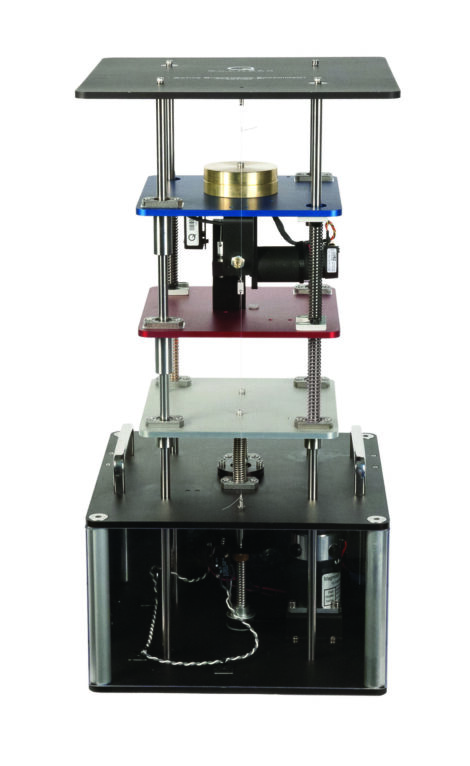
\includegraphics[width=0.48\textwidth]{lab}
    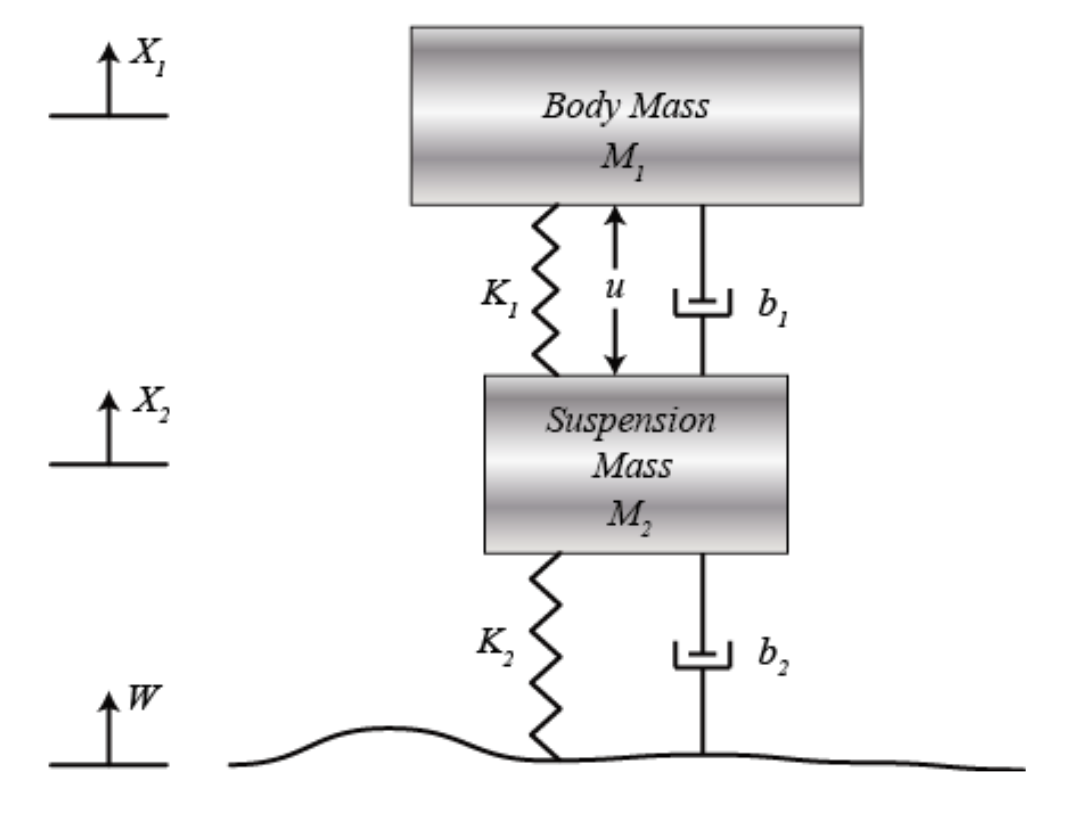
\includegraphics[width=0.48\textwidth]{suspension}
    \caption{Aktif süspansiyon sistemi ve modeli}\label{fig:suspension}
\end{figure}
\begin{table}[!htb]
    \centering
    \begin{tabular}{ccc}\hline
        \textbf{Açıklama}&\textbf{Değişken}& \textbf{Değer}\\\hline
        Gövde kütlesi&$m_s$& 2.45  \\
        Süspansiyon kütlesi&$m_{us}$& 1   \\
        Süspansiyon yay sabiti&$k_s$& 900 \\  
        Teker yay sabiti&$k_{us}$& 1250 \\
        Süspansiyon damper katsayısı&$b_s$& 7.5 \\
        Teker damper katsayısı&$b_{us}$& 5 \\  \hline
    \end{tabular}
    \caption{Süspansiyon modeli parametreleri}
\end{table}
\noindent\textbf{Çözüm:} 
Birinci dereceden türev
\begin{equation}
    \frac{dx}{dt}=\frac{x(k)-x(k-1)}{T}
\end{equation}
olarak ayrıklaştırılabilir. Bu durumda denklemler
\begin{equation}
\begin{split}
    \frac{x_1(k)-x_1(k-1)}{T}&=x_2(k-1)-x_4(k-1)\\
    \frac{x_2(k)-x_2(k-1)}{T}&=\frac{-k_s}{m_s}x_1(k-1)-\frac{b_s}{m_s}x_2(k-1)+\frac{b_s}{m_s}x_4(k-1)+\frac{1}{m_s}w(k-1)+\frac{1}{m_s}u(k-1)\\
    \frac{x_3(k)-x_3(k-1)}{T}&=x_4(k-1)\\
    \frac{x_4(k)-x_4(k-1)}{T}&=\frac{k_s}{m_{us}}x_1(k-1)+\frac{b_s}{m_{us}}x_2(k-1)-\frac{k_{us}}{m_{us}}x_3(k-1)-\frac{b_s+b_{us}}{m_{us}}x_4(k-1)-\frac{1}{m_{us}}w(k-1)-\frac{1}{m_{us}}u(k-1)
\end{split}
\end{equation}
ve
\begin{equation}
\begin{split}
x_1(k)&=x_1(k-1)+Tx_2(k-1)-Tx_4(k-1)\\
x_2(k)&=\frac{-k_sT}{m_s}x_1(k-1)+\frac{m_s-b_sT}{m_s}x_2(k-1)+\frac{b_sT}{m_s}x_4(k-1)+\frac{T}{m_s}u(k-1)\\
x_3(k)&=x_3(k-1)+Tx_4(k-1)-Tw(k-1)\\
x_4(k)&=\frac{k_sT}{m_{us}}x_1(k-1)+\frac{b_sT}{m_{us}}x_2(k-1)-\frac{k_{us}T}{m_{us}}x_3(k-1)+\frac{m_{us}-b_sT-b_{us}T}{m_{us}}x_4(k-1)+\frac{b_{us}T}{m_{us}}w(k-1)-\frac{T}{m_{us}}u(k-1)
\end{split}
\end{equation}
olarak yazılabilmektedir. Değerler yerine yazılırsa
\begin{equation}
    \begin{split}
    x_1(k)&=x_1(k-1)+0.001x_2(k-1)-0.001x_4(k-1)\\
    x_2(k)&=-0.36x_1(k-1)+0.997x_2(k-1)+0.003x_4(k-1)\\
    x_3(k)&=x_3(k-1)+0.001x_4(k-1)-0.001w(k-1)\\
    x_4(k)&=0.9x_1(k-1)+0.0075x_2(k-1)-1.25x_3(k-1)+0.9875x_4(k-1)+0.005w(k-1)
    \end{split}
\end{equation}

\noindent\textbf{Extra:}Fark denklemlerini kullanarak $u$ girişine sıfır ve $w=0.04sin(2\pi10t)$ uygulayınız ve $x_1$, $x_2$, $x_3$ ve $x_4$ değişkenlerini çiziniz. Çizimi $0-1\,s$ arasında oluşturunuz. 
\begin{figure}[!htb]
    \centering
    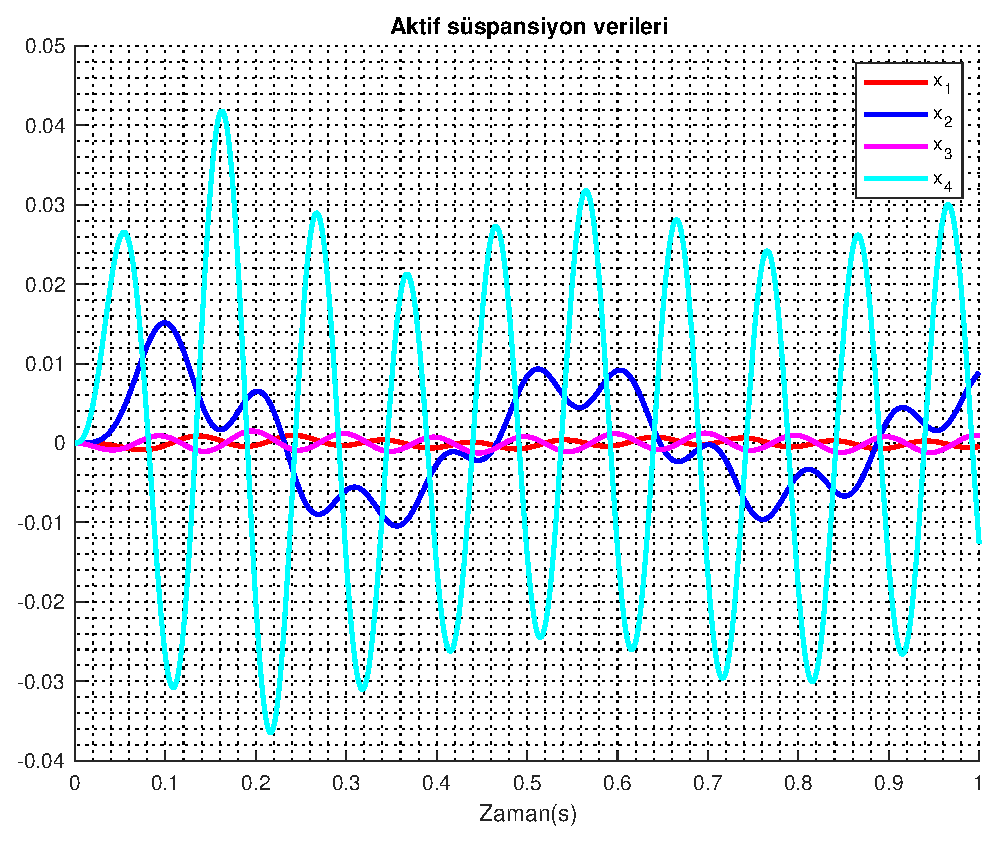
\includegraphics[width=0.75\textwidth]{plot1}
    \caption{Extra soru için elde edilen çizim}
    \label{fig:plot1}
\end{figure}